\section{Evaluación}

\begin{frame}[t]{Plataforma de evaluación}
\begin{itemize}
  \item \textenum{Plataforma}:
    \begin{itemize}
      \item 2 $\times$ Intel Xeon Ivy Bridge E5-2695 v2.
      \item Total number of cores $Rightarrow$ 24.
      \item Clock frequency: 2.40 GHz.
      \item L3 cache size $Rightarrow$ 30 MB.
      \item Main memory: 128 GB DDR3.
      \item OS: Ubuntu Linux 14.04 LTS, kernel 3.13.
    \end{itemize}

  \vfill
  \item \textenum{Compilador}: GCC 5.0.
    \begin{itemize}
      \item OpenMP: incluido en GCC.
      \item ISO C++ Threads: includa en biblioteca estándar de GCC.
      \item Intel TBB: \textgood{\url{www.threadingbuildingblocks.org}}
    \end{itemize}
\end{itemize}
\end{frame}

\begin{frame}[t]{Benchmark ejemplo}
\begin{itemize}
  \item Procesamiento de video para detección de bordes con dos filtros aplicados a cada imagen.
    \begin{itemize}
      \item Desenfoque gausiano.
      \item Sobel.
    \end{itemize}
  \vfill\pause
  \item Una buena aplicación del patrón \textgood{pipeline}:
    \begin{itemize}
      \item S1: Lectura de fotogramas.
      \item S2: Desenfoque gausiano (puede aplicarse \textgood{farm}).
      \item S3: Filtro de Sobel (puede aplicarse \textgood{farm}).
      \item S4: Escritara de fotogramas.
    \end{itemize}
  \vfill\pause
  \item \textenum{Enfoques}:
    \begin{itemize}
      \item Paralelización manual.
      \item \textmark{GrPPI}.
    \end{itemize}
\end{itemize}
\end{frame}

\begin{frame}{Esfuerzo de paralelización}
\begin{tabular}{|c|r|r|r|r|}
\hline
composición& \multicolumn{4}{c|}{\centering\let\newline\\ \% de incremento de líneas de código} \\\cline{2-5}
de pipeline& \textbf{C++ Threads}  & \textbf{OpenMP} & \textbf{Intel TBB}  & \textbf{GrPPI} \\\hline\hline
\texttt{(\,p\,$|$\,p\,$|$\,p\,$|$\,p\,)} & $+$8.8\,\%   & $+$13.0\,\%  & $+$25.9\,\% & $+$1.8\,\% \\
\texttt{(\,p\,$|$\,f\,$|$\,p\,$|$\,p\,)} & $+$59.4\,\%  & $+$62.6\,\%  & $+$25.9\,\% & $+$3.1\,\% \\
\texttt{(\,p\,$|$\,p\,$|$\,f\,$|$\,p\,)} & $+$60.0\,\%  & $+$63.9\,\%  & $+$25.9\,\% & $+$3.1\,\% \\
\texttt{(\,p\,$|$\,f\,$|$\,f\,$|$\,p\,)} & $+$106.9\,\% & $+$109.4\,\% & $+$25.9\,\% & $+$4.4\,\% \\\hline
\end{tabular}
\end{frame}

\begin{frame}{Rendimiento: Fotogramas por segundo}
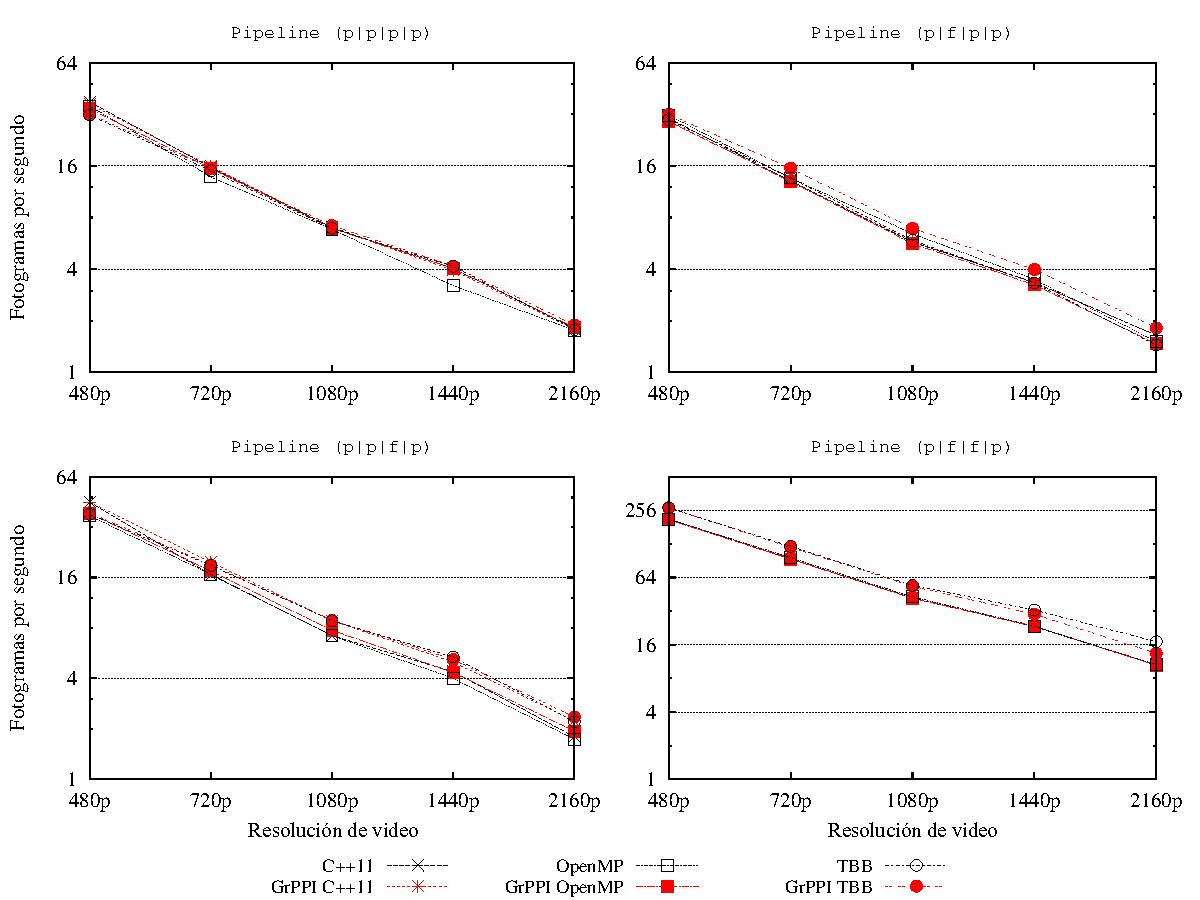
\includegraphics[height=.85\textheight]{fps.pdf}
\end{frame}

\begin{frame}{Observaciones}
\begin{itemize}
  \item Impacto del patrón \textgood{farm}:
    \begin{itemize}
      \item El uso de \textgood{farm} en ambas etapas causa una mejora sustancial del rendimiento.
        \begin{itemize}
          \item Equilibrio.
        \end{itemize}
      \item El uso de \textgood{farm} en una única etapa del pipeline no tiene impacto significativo.
        \begin{itemize}
          \item Desequilibrio.
        \end{itemize}
    \end{itemize}

  \vfill\pause
  \item Impacto de GrPPI en el rendimento.
    \begin{itemize}
      \item Sobrecoste por debajo del 2\%.
    \end{itemize}

  \vfill\pause
  \item Impacto en el esfuerzo.
    \begin{itemize}
      \item Reducción significativa con respecto a los otros enfoques de programación.
    \end{itemize}
\end{itemize}
\end{frame}

\begin{frame}[t]{Conclusiones}
\begin{itemize}
  \item GrPPI permite cambiar de modelo de programación subyacente con mínimo esfuerzo
        gracias al uso de C++ moderno.
  \vfill\pause
  \item Diseño compacto para ocultar la complejidad de alternativas de implementación.
  \vfill\pause
  \item Soporte de múltiples patrones:
    \begin{itemize}
      \item \textenum{Datos}: \textmark{map}, \textmark{reduce}, \textmark{map/reduce}, \textmark{stencil}.
      \item \textenum{Tareas}: \textmark{divide/conquer}.
      \item \textenum{streaming} \textmark{pipeline} con etapas \textmark{farm}, \textmark{filter}, \textmark{reduce},
                                 \textmark{iteration}.
    \end{itemize}
  \vfill\pause
  \item Mínimo sobrecoste de:
    \begin{itemize}
      \item Modificaciones del código fuente.
      \item Rendimiento.
    \end{itemize}
\end{itemize}
\end{frame}

\begin{frame}[t]{Trabajo futuro}
\begin{itemize}
  \item Mejorar y ampliar políticas de ejecución (Thrust, FastFlow, \ldots).
  \item Incorporar nuevos patrones.
  \item Extender y simplificar la interfaz para patrones de datos.
  \item Dar soporte a combinación de políticas de ejecución.
  \item Mejorar el soporte NUMA.
  \item Ampliar aplicaciones ejemplo y benchmarks.
  \vfill
  \item \textgood{\url{www.githb.com/arcosuc3m/grppi}}.
\end{itemize}
\end{frame}
